\section{Modelo de Entidad Relación y Modelo Relacional}

A continuación, se mostrarán el Modelo de Entidad Relación y el Modelo Relacional correspondientes a nuestra solución del problema.\\

\subsection{Modelo de Entidad Relación}


\begin{center}
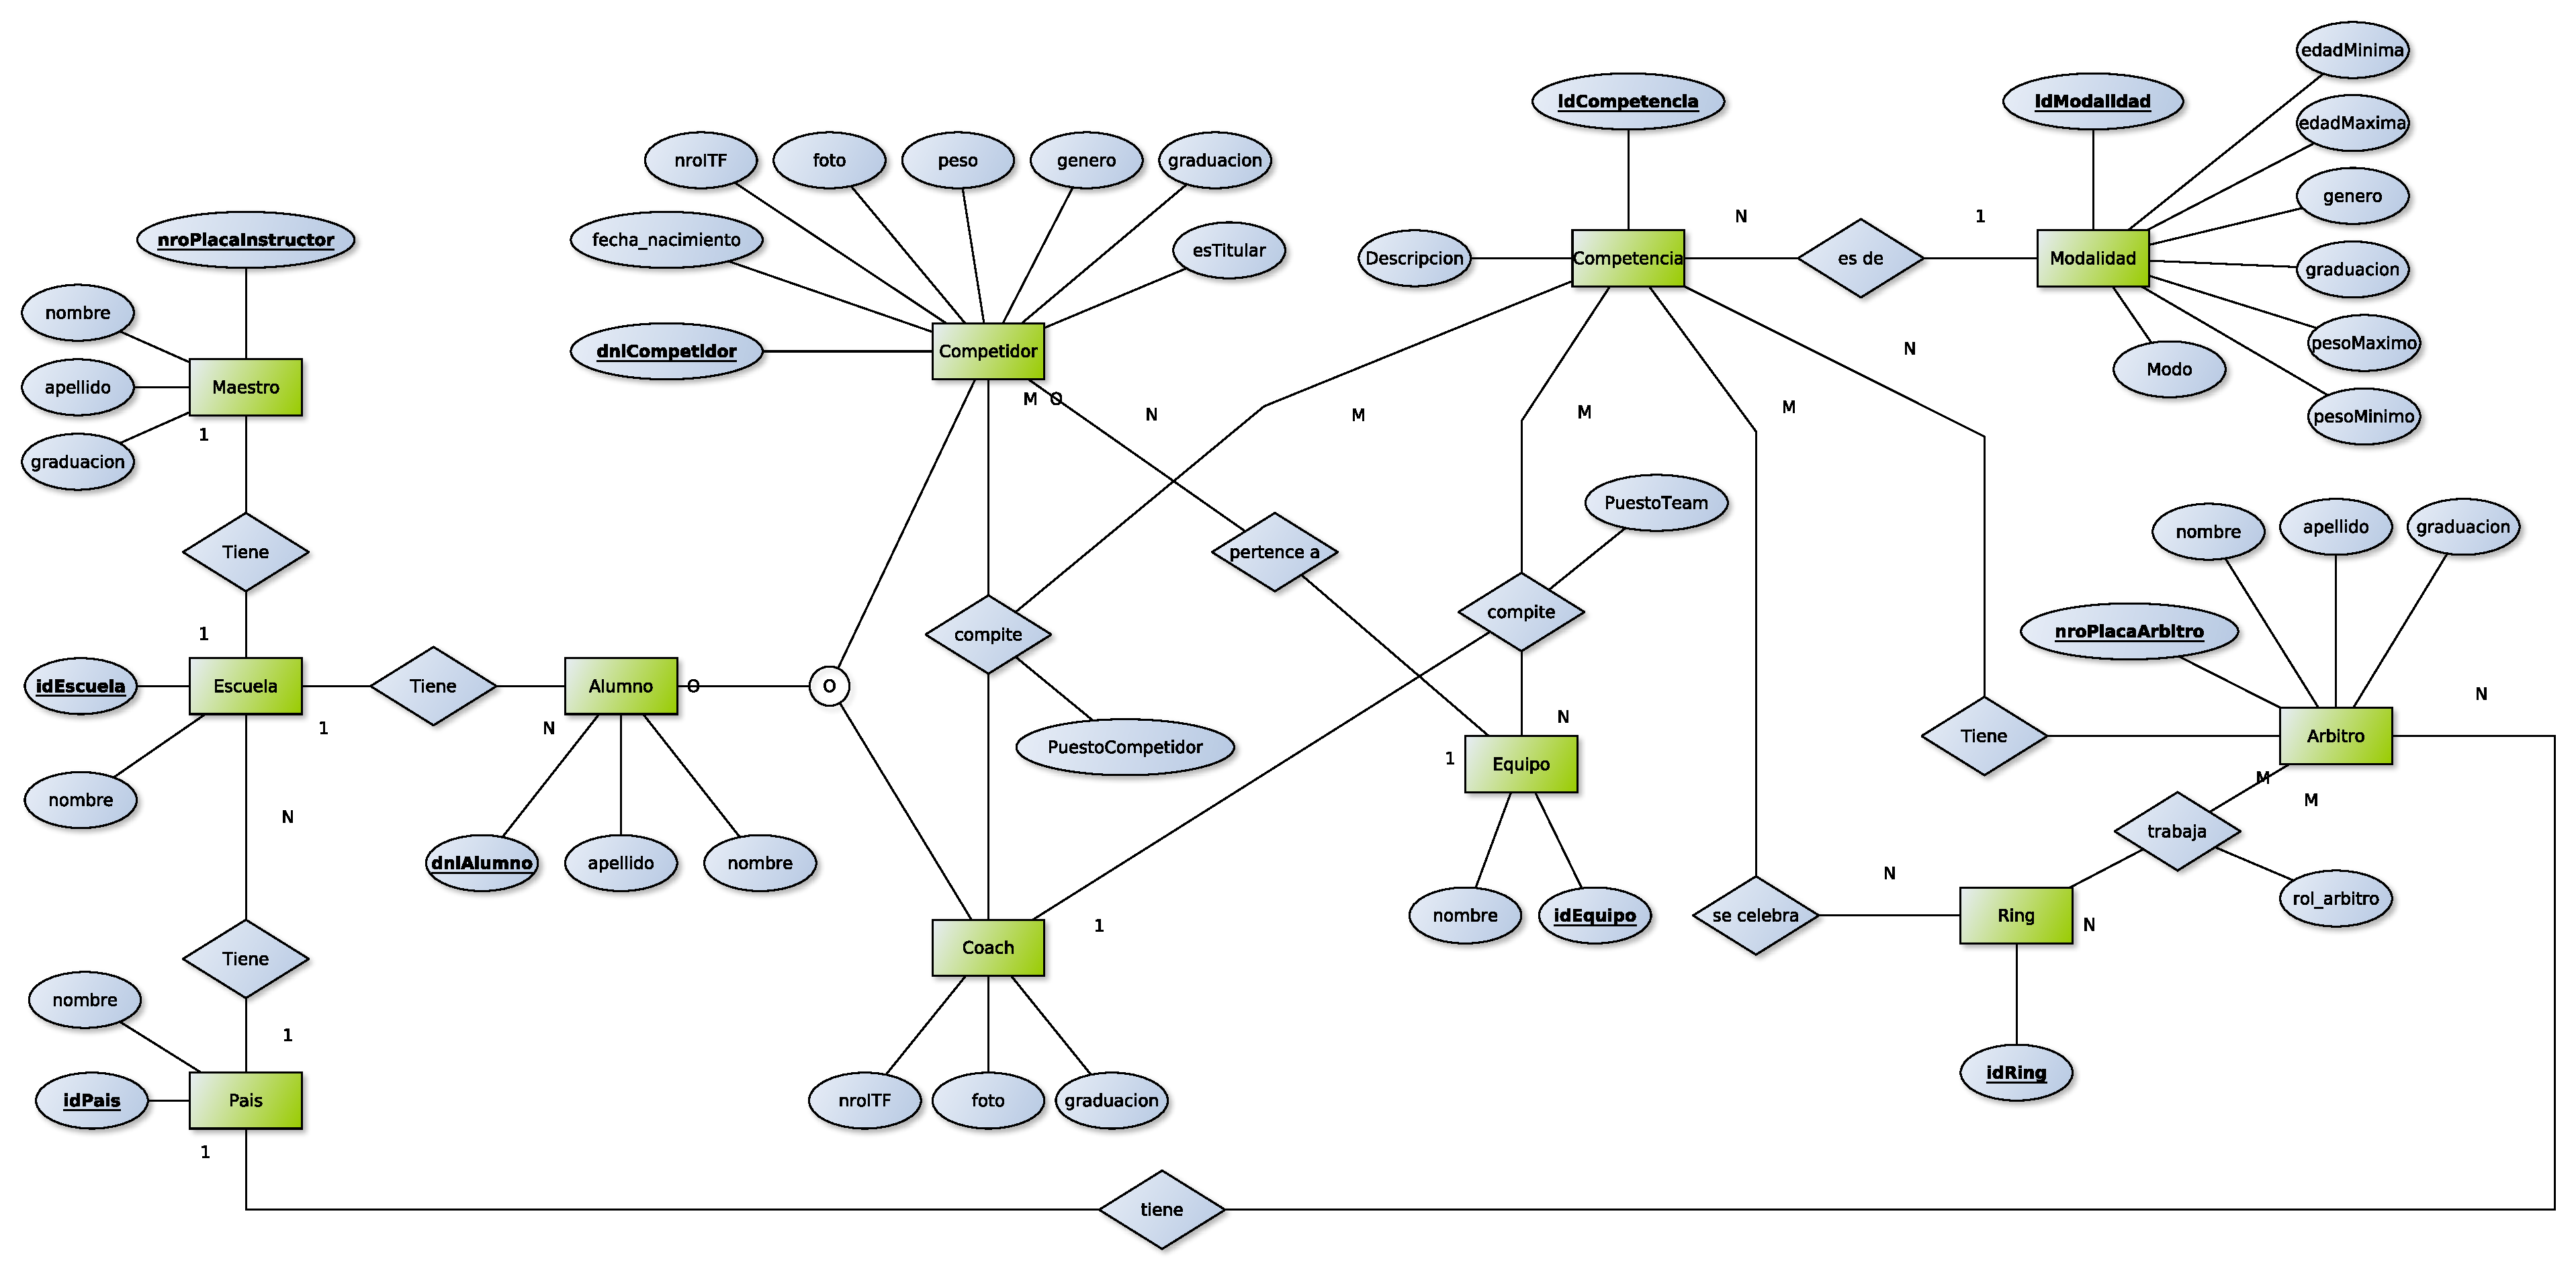
\includegraphics[width=20cm,keepaspectratio,angle=90]{./imagenes/DER.pdf}\newline
\end{center}

\newpage
\subsection{Modelo Relacional}

\noindent\textbf{Escuela}(\uline{idEscuela}, nombre, \dashuline{idPais}, \dashuline{nroPlacaInstructor}) 
\\
\\
PK = CK = \{ idEscuela \} \\
FK = \{ idPais, nroPlacaInstructor \} \\

\begin{verbatim}
--------------------------------------------------------------------------
\end{verbatim}

\noindent\textbf{Pais}(\uline{idPais}, nombre)
\\
\\
PK = CK = \{ idPais \} \\


\begin{verbatim}
--------------------------------------------------------------------------
\end{verbatim}

\noindent\textbf{Maestro}(\uline{nroPlacaInstructor}, nombre, apellido, graduación)
\\
\\
PK = CK = \{ nroPlacaInstructor \} \\


\begin{verbatim}
--------------------------------------------------------------------------
\end{verbatim}

\noindent\textbf{Alumno}(\uline{dniAlumno}, nombre, apellido, \dashuline{idEscuela})
\\
\\
PK = CK = \{ dniAlumno \} \\
FK = \{ idEscuela \} \\

\textit{Restricciones:}
\begin{itemize}
	\item un Alumno puede ser coach y competidor a la vez.
\end{itemize}

\begin{verbatim}
--------------------------------------------------------------------------
\end{verbatim}

\noindent\textbf{Coach}(\uuline{dniAlumno}, nroITF, foto, graduación)
\\
\\
PK = CK = FK = \{ dniAlumno \} \\

\textit{Restricciones:}
\begin{itemize}
	\item Un alumno puede \textbf{no} estar en Coach
	\item habrá al menos un coach por cada 5 competidores
\end{itemize}


\begin{verbatim}
--------------------------------------------------------------------------
\end{verbatim}

\noindent\textbf{Competidor}(\uuline{dniAlumno}, nroITF, fechaNacimiento, género, graduación, peso, foto, esTitular, \dashuline{idEquipo})
\\
\\
PK = CK = \{ dniCompetidor \} \\
FK = \{ idEquipo \} \\


\textit{Restricciones:}
\begin{itemize}
	\item Un alumno puede \textbf{no} estar en Competidor.
	\item El Competidor puede \textbf{no} estar en Equipo.
	\item Si el Competidor está en Equipo, entonces si es titular, el campo esTitular tendrá un True, y si es suplente tendrá un false. En caso de no tener equipo, ese campo contendrá null.
\end{itemize}

\begin{verbatim}
--------------------------------------------------------------------------
\end{verbatim}

\noindent\textbf{Equipo}(\uline{idEquipo}, nombre)
\\
\\
PK = CK = \{ idEquipo \} \\

\textit{Restricciones:}
\begin{itemize}
	\item Los equipos están conformados por 5 titulares y 3 suplentes, y todos deben ser de la misma escuela.
\end{itemize}


\begin{verbatim}
--------------------------------------------------------------------------
\end{verbatim}

\noindent\textbf{Competencia}(\uline{idCompetencia}, descripcion, \dashuline{idModalidad})
\\
\\
PK = CK = \{ idCompetencia \} \\
FK = \{ idModalidad \} \\

\begin{verbatim}
--------------------------------------------------------------------------
\end{verbatim}

\noindent\textbf{compiteEnCompetenciaInd}(\uuline{dniCompetidor}, \uuline{idCompetencia}, \dashuline{dniCoach}, puestoCompetidor)
\\
\\
PK = \{ (dniCompetidor,idCompetencia) \} \\
CK = \{ (dniCompetidor,idCompetencia), (dniCompetidor,dniCoach), (idCompetencia,dniCoach)\} \\
FK = \{ dniCompetidor, idCompetencia, dniCoach \} \\

\textit{Restricciones:}
\begin{itemize}
	\item Los competidores que se registren en una competencia, deben cumplir con las exigencias de la misma, es decir, deben respetar la edad, el sexo, la graduación, o cualquier exigencia que la modalidad de la competencia exija.
	\item Un coach que es competidor no podrá ser coach de si mismo.
\end{itemize}


\begin{verbatim}
--------------------------------------------------------------------------
\end{verbatim}

\noindent\textbf{compiteEnCompetenciaTeam}(\uuline{idEquipo}, \uuline{idCompetencia}, \dashuline{dniCoach}, puestoTeam)
\\
\\
PK = \{ (idEquipo,idCompetencia) \} \\
CK = \{ (idEquipo,idCompetencia), (idEquipo,idCompetencia), (idCompetencia,dniCoach)\} \\
FK = \{ idEquipo, idCompetencia, dniCoach \} \\

\textit{Restricciones:}
\begin{itemize}
	\item Los competidores de los equipos que se registren en una competencia, deben cumplir con las exigencias de la misma, es decir, deben respetar la edad, el sexo, la graduación, o cualquier exigencia que la modalidad de la competencia exija.
	\item Un coach que es competidor no podrá ser coach del equipo al que pertenece.
\end{itemize}

\begin{verbatim}
--------------------------------------------------------------------------
\end{verbatim}

\noindent\textbf{Modalidad}(\uline{idModalidad}, edadMínima, edadMáxima, género, graduación, pesoMínimo, pesoMáximo, modo)
\\
\\
PK = CK = \{ idModalidad \} \\
\textit{Restricciones:}
\begin{itemize}
	\item Los modos determinan que atributos deben estar en null según lo pedido en el enunciado.
\end{itemize}


\begin{verbatim}
--------------------------------------------------------------------------
\end{verbatim}

\noindent\textbf{Ring}(\uline{idRing})
\\
\\
PK = CK = \{ idRing \} \\

\begin{verbatim}
--------------------------------------------------------------------------
\end{verbatim}

\noindent\textbf{Arbitro}(\uline{nroPlacaArbitro}, nombre, apellido, graduación, \dashuline{idPais})
\\
\\
PK = CK = \{ nroPlacaArbitro \} \\
FK = \{ idPais \} \\

\begin{verbatim}
--------------------------------------------------------------------------
\end{verbatim}

\noindent\textbf{arbitrosEnCompetencias}(\uuline{nroPlacaArbitro}, \uuline{idCompetencia})
\\
\\
PK = CK = FK = \{ (nroPlacaArbitro,idCompetencia) \} \\

\textit{Restricciones:}
\begin{itemize}
	\item La graduación de un arbitro debe ser siempre MAYOR a la graduación de la modalidad de la competencia.
\end{itemize}

\begin{verbatim}
--------------------------------------------------------------------------
\end{verbatim}

\noindent\textbf{ringsDeCompetencias}(\uuline{idRing}, \uuline{idCompetencia})
\\
\\
PK = CK = FK = \{ (idRing,idCompetencia) \} \\

\textit{Restricciones:}
\begin{itemize}
	\item Los rings de cada competencia deben poseer arbitros que tengan la capacidad de dirigirlas.
\end{itemize}

\begin{verbatim}
--------------------------------------------------------------------------
\end{verbatim}

\noindent\textbf{puestoArbitroEnRing}(\uuline{nroPlacaArbitro},\uuline{idRing}, puesto)
\\
\\
PK = CK = FK = \{ (nroPlacaArbitro,idRing) \} \\

\textit{Restricciones:}
\begin{itemize}
	\item En un Ring siempre habrá un presidente de mesa, un arbitro central, varios jueces y al menos tres suplentes.
\end{itemize}

\begin{verbatim}
--------------------------------------------------------------------------
\end{verbatim}